\documentclass[a4paper, twoside]{report}

\usepackage[english]{babel}
\usepackage[utf8]{inputenc}
\usepackage[T1]{fontenc}
\usepackage{listings}
\usepackage{hyperref}
\hypersetup{colorlinks=false}
\usepackage{lscape}
\usepackage{subfigure}
\usepackage{amsmath}
\usepackage{graphicx}
\usepackage[colorinlistoftodos]{todonotes}
\usepackage[backend=biber]{biblatex}

\DeclareMathOperator{\relu}{ReLU}
\DeclareMathOperator{\softmax}{softmax}

\addbibresource{bibs/references.bib}

%% Sets page size and margins
\usepackage[a4paper,top=3cm,bottom=2cm,left=3cm,right=3cm,marginparwidth=1.75cm]{geometry} 

\title{Semi-supervised graph node classification of CORA dataset using GCN}
\author{Junghyun Lee}
% Update supervisor and other title stuff in title/title.tex

\begin{document}
\begin{titlepage}

\newcommand{\HRule}{\rule{\linewidth}{0.5mm}} % Defines a new command for the horizontal lines, change thickness here

%----------------------------------------------------------------------------------------
%	LOGO SECTION
%----------------------------------------------------------------------------------------

\includegraphics[width=8cm]{title/logo.png}\\[1cm] % Include a department/university logo - this will require the graphicx package
 
%----------------------------------------------------------------------------------------

\center % Center everything on the page

%----------------------------------------------------------------------------------------
%	HEADING SECTIONS
%----------------------------------------------------------------------------------------
\quad\\[1.5cm]
%\textsc{\LARGE MSc Thesis}\\[1.5cm] % Name of your university/college
\textsc{\Large Korea Advanced Institute of Technology}\\[0.5cm] % Major heading such as course name
\textsc{\large Department of Mathematical Sciences}\\[0.5cm] % Minor heading such as course title

%----------------------------------------------------------------------------------------
%	TITLE SECTION
%----------------------------------------------------------------------------------------
\makeatletter
\HRule \\[0.4cm]
{ \huge \bfseries \@title}\\[0.4cm] % Title of your document
\HRule \\[1.5cm]
 
%----------------------------------------------------------------------------------------
%	AUTHOR SECTION
%----------------------------------------------------------------------------------------

\begin{minipage}{0.4\textwidth}
\begin{flushleft} \large
\emph{Author:}\\
\@author % Your name
\end{flushleft}
\end{minipage}
~
\begin{minipage}{0.4\textwidth}
\begin{flushright} \large
\emph{Instructor:} \\
Prof. Chang Dong Yoo 
% Uncomment the following lines if there's a co-supervisor
%\\[1.2em] % Supervisor's Name
%\emph{Co-Supervisor:} \\
%Dr. Adam Smith % second marker's name
\end{flushright}
\end{minipage}\\[3cm]
\makeatother


%----------------------------------------------------------------------------------------
%	DATE SECTION
%----------------------------------------------------------------------------------------

{\large Homework \#4}\\[0.5cm]
{\large \emph{EE531: Statistical Learning Theory, Fall 2019}}\\[0.5cm]
{\large \today}\\[2cm] % Date, change the \today to a set date if you want to be precise

\vfill % Fill the rest of the page with whitespace

\end{titlepage}

\begin{abstract}
In this homework, I have implemented a simple version of GCN(Graph Convolutional Network) to do a semi-supervised graph node classification of CORA dataset.
The algorithm is based upon the work by Kipf \& Welling, 2016.

(Coding done in Google Colaboratory.)
\end{abstract}
 
\tableofcontents

\chapter{Implementation}
Implementation was done using the Google Colaboratory. All the modifications that I've done to the original template are accompanied by the comments that I've put.

Below, I've added additional explanations for some of the features that I've used or modified.


\section{Initialization}

I have initialized some boolean parameters to be used later on for the training/evaluation/testing.

\begin{figure}[htbp]
\centering
\includegraphics[width=0.6\linewidth]{implementation/fig/code0.png}
\caption{Initialization}
\label{fig:code0}
\end{figure}

\section{TensorBoardColab}

{\bf TensorBoard} is a visualization toolkit that supports various experimentation. Especially, it is useful in tracking and visualizing metrics such as loss and accuracy.

It is supported in multiple platforms, including Tensorflow, Google Colaboratory...etc.

\begin{figure}[htbp]
\centering
\includegraphics[width=0.6\linewidth]{implementation/fig/code1.png}
\caption{TensorBoardColab}
\label{fig:code1}
\end{figure}


\section{GraphConvolutionLayer}

\subsection{Parameter Initialization}

Here I have given myself two choices for initializing weights:
\begin{enumerate}
\item Sampling from $U \left(-\frac{1}{\sqrt{m}}, \frac{1}{\sqrt{m}}\right)$\cite{Goodfellow2016}
\item Xavier initialization\cite{Glorot2010}
\end{enumerate}

For either case, bias was initialized by sampling from $U \left(-\frac{1}{\sqrt{m}}, \frac{1}{\sqrt{m}}\right)$.

\begin{figure}[htbp]
\centering
\includegraphics[width=0.6\linewidth]{implementation/fig/code2.png}
\caption{Parameter initialization}
\label{fig:code2}
\end{figure}

\subsection{Forward Function}

For forward propagation, I have used the heuristic of
$$forward(H) = A H W + b$$
where $A$ is the adjacency matrix, $H$ is the input matrix, $W$ is the weight matrix, and $b$ is the bias matrix.

\begin{figure}[htbp]
\centering
\includegraphics[width=0.6\linewidth]{implementation/fig/code3.png}
\caption{Forward propagation}
\label{fig:code3}
\end{figure}

\section{GCN}

\subsection{Network Initialization}

Following the work of Kipf \& Welling\cite{Kipf2017}, I have decided to implemented the two-layered GCN. To do that, two {\it GraphConvolutionLayer}'s, along with {\it dropout}, were initialized.

\begin{figure}[htbp]
\centering
\includegraphics[width=0.6\linewidth]{implementation/fig/code4.png}
\caption{Network initialization}
\label{fig:code4}
\end{figure}

\subsection{Forward Function}

I have used the forward model of the form:
$$forward(X, A) = \softmax\left(\hat{A}  \relu\left( \hat{A} X W^{(0)} \right) W^{(1)} \right)$$

\begin{figure}[htbp]
\centering
\includegraphics[width=0.6\linewidth]{implementation/fig/code5.png}
\caption{Forward propagation}
\label{fig:code5}
\end{figure}

\section{Training/Validation/Testing}

(Even though I only describe one of the three here, the rest are the same. Just change the index set to the appropriate one.)

I have utilized the negative log likelihood loss. Also, I have updated the tensorboard plot for every epoch.

\begin{figure}[htbp]
\centering
\includegraphics[width=0.6\linewidth]{implementation/fig/code6.png}
\caption{Training phase}
\label{fig:code6}
\end{figure}

\section{Confusion Matrix}

For the confusion matrix plot, I have utilized the external github open repository: \url{https://github.com/wcipriano/pretty-print-confusion-matrix}.

\begin{figure}[htbp]
\centering
\includegraphics[width=0.6\linewidth]{implementation/fig/code7.png}
\caption{Confusion matrix}
\label{fig:code7}
\end{figure}
\chapter{Results}
%For my evaluation, I've used {\bf Tensorboard} for plotting the learning(loss) curve and performance(accuracy) curve for both training and validating processes. Also, I've used external open source library({\bf pretty-print-confusion-matrix}\footnote{\url{https://github.com/wcipriano/pretty-print-confusion-matrix}}) for plotting the confusion matrix for the test set.
Here,
\begin{itemize}
\item Original model: One with uniform initialization with dropouts(rate=0.5).

\item Ver. 1: Original model with Xavier (Uniform) Initialization

\item Ver. 2: Original model without dropouts

\item Ver. 3: Original model with Xavier Initialization and without dropouts
\end{itemize}

In all the plots, x-axis corresponds to the epoch.
As for the graphs,

\begin{itemize}
\item Accuracy graph
	\begin{itemize}
	\item Dark red: train accuracy
	\item Bright red: validation accuracy
	\end{itemize}

\item Loss graph
	\begin{itemize}
	\item Dark blue: train loss
	\item Bright blue: validation loss
	\end{itemize}
\end{itemize}

\newpage
\section{Original model}

\begin{figure}[htbp]
\centering
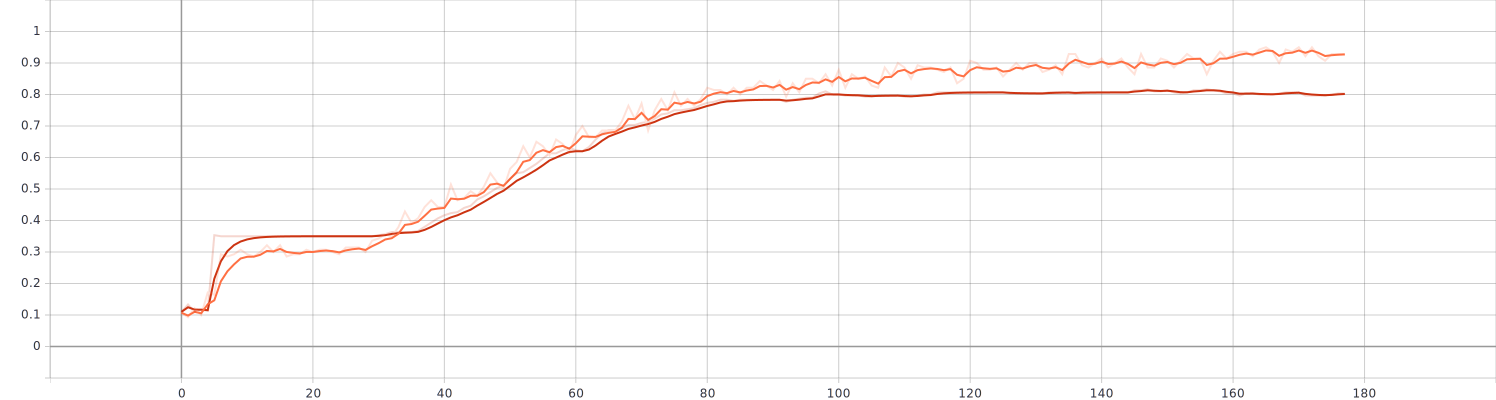
\includegraphics[width=0.7\linewidth]{results/fig/Accuracy0.png}
\caption{Accuracy graph}
\label{fig:accuracy0}
\end{figure}

\begin{figure}[htbp]
\centering
\includegraphics[width=0.7\linewidth]{results/fig/Loss0.png}
\caption{Loss graph}
\label{fig:evaluation0}
\end{figure}

\begin{figure}[htbp]
\centering
\includegraphics[width=0.6\linewidth]{results/fig/confusion0.png}
\caption{Confusion matrix}
\label{fig:confusion0}
\end{figure}

\newpage
\section{Modified Model (Ver. 1)}

\begin{figure}[htbp]
\centering
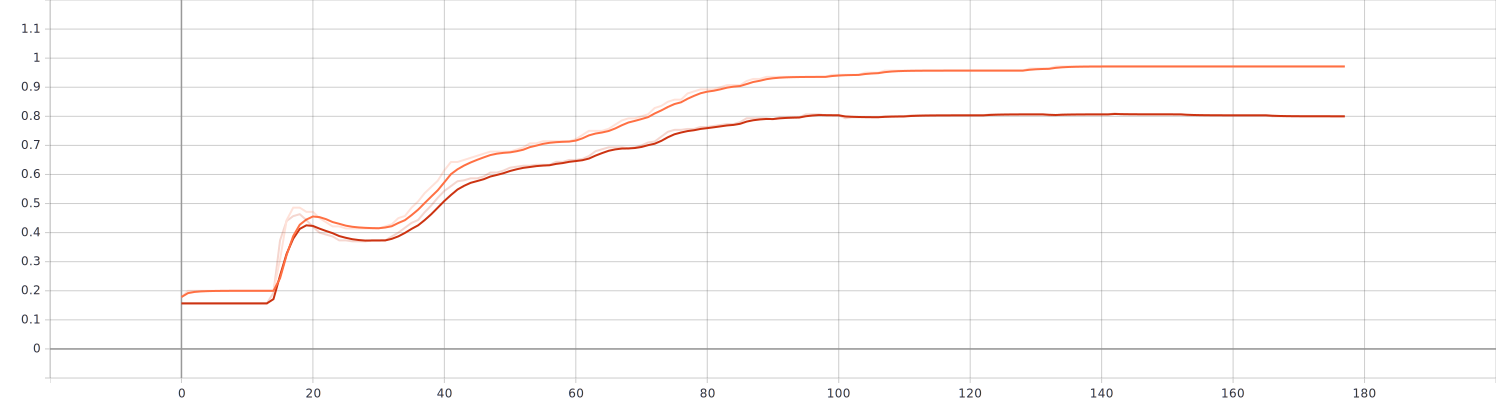
\includegraphics[width=0.7\linewidth]{results/fig/Accuracy1.png}
\caption{Accuracy graph}
\label{fig:accuracy1}
\end{figure}

\begin{figure}[htbp]
\centering
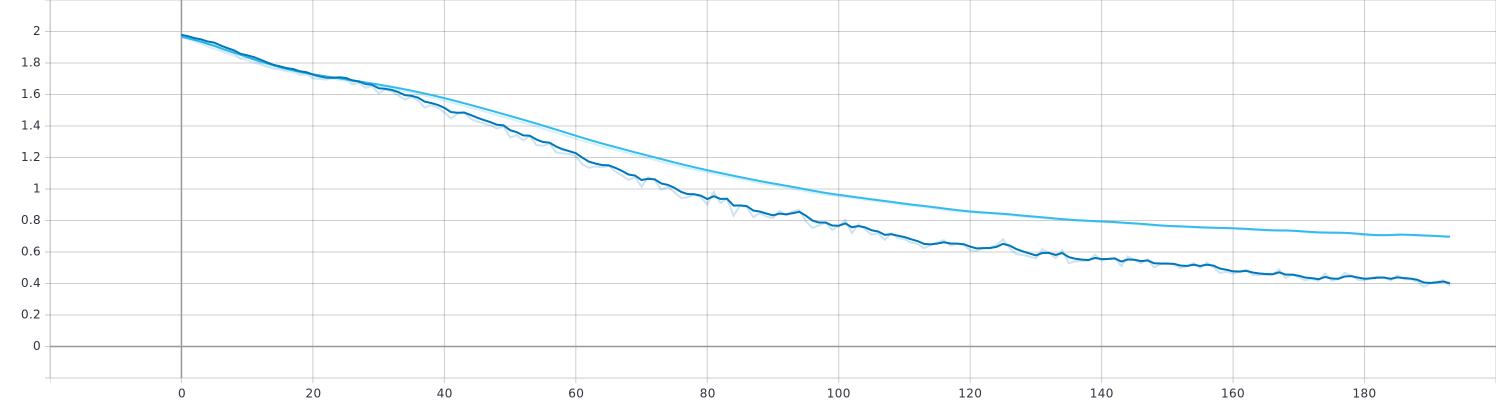
\includegraphics[width=0.7\linewidth]{results/fig/Loss1.png}
\caption{Loss graph}
\label{fig:evaluation1}
\end{figure}

\begin{figure}[htbp]
\centering
\includegraphics[width=0.6\linewidth]{results/fig/confusion1.png}
\caption{Confusion matrix}
\label{fig:confusion1}
\end{figure}

\newpage
\section{Modified Model (Ver. 2)}

\begin{figure}[htbp]
\centering
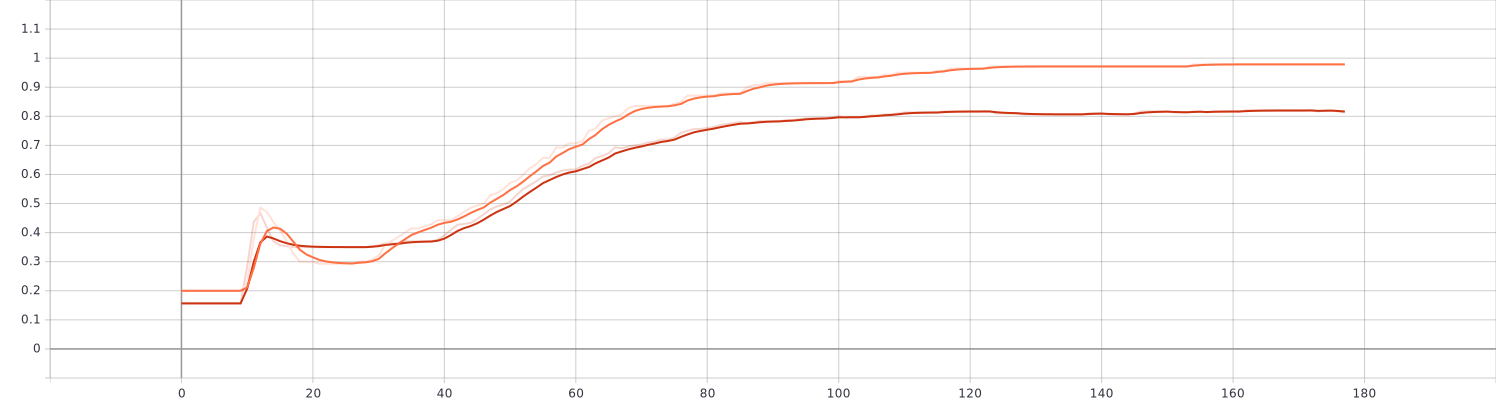
\includegraphics[width=0.7\linewidth]{results/fig/Accuracy2.png}
\caption{Accuracy graph}
\label{fig:accuracy2}
\end{figure}

\begin{figure}[htbp]
\centering
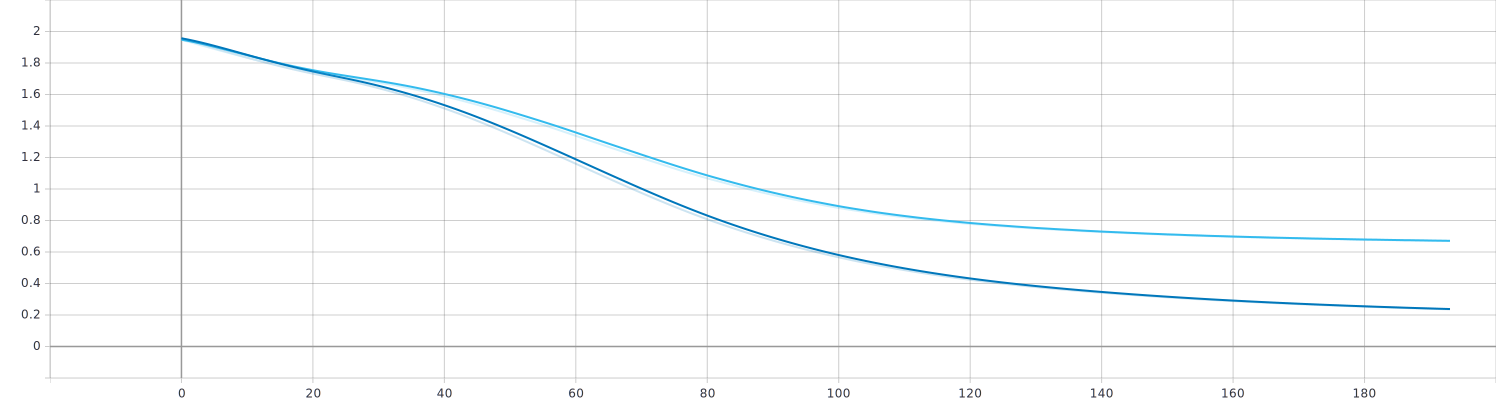
\includegraphics[width=0.7\linewidth]{results/fig/Loss2.png}
\caption{Loss graph}
\label{fig:evaluation2}
\end{figure}

\begin{figure}[htbp]
\centering
\includegraphics[width=0.6\linewidth]{results/fig/confusion2.png}
\caption{Confusion matrix}
\label{fig:confusion2}
\end{figure}

\newpage
\section{Modified Model (Ver. 3)}

\begin{figure}[htbp]
\centering
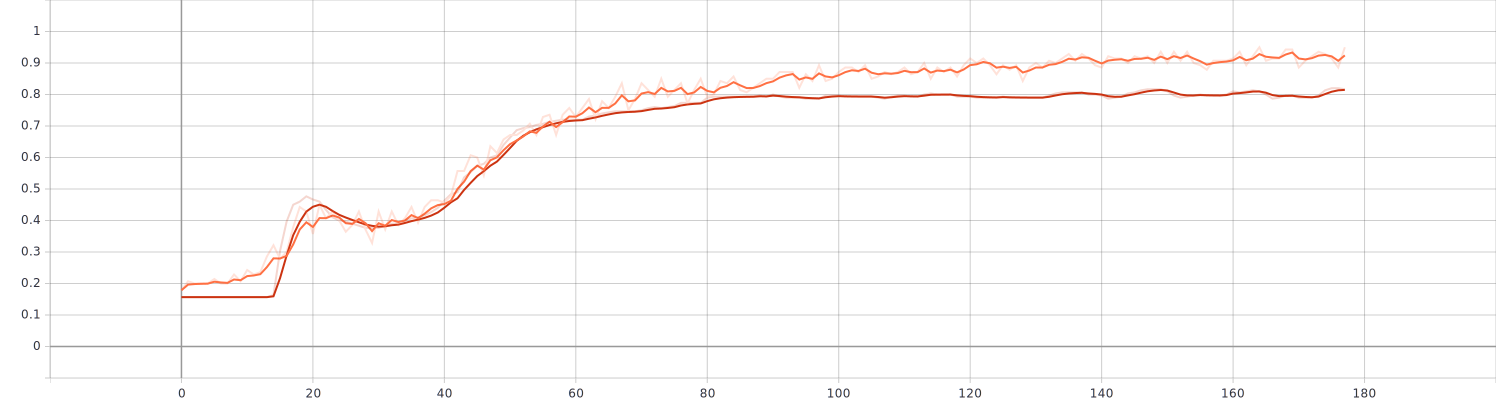
\includegraphics[width=0.7\linewidth]{results/fig/Accuracy3.png}
\caption{Accuracy graph}
\label{fig:accuracy3}
\end{figure}

\begin{figure}[htbp]
\centering
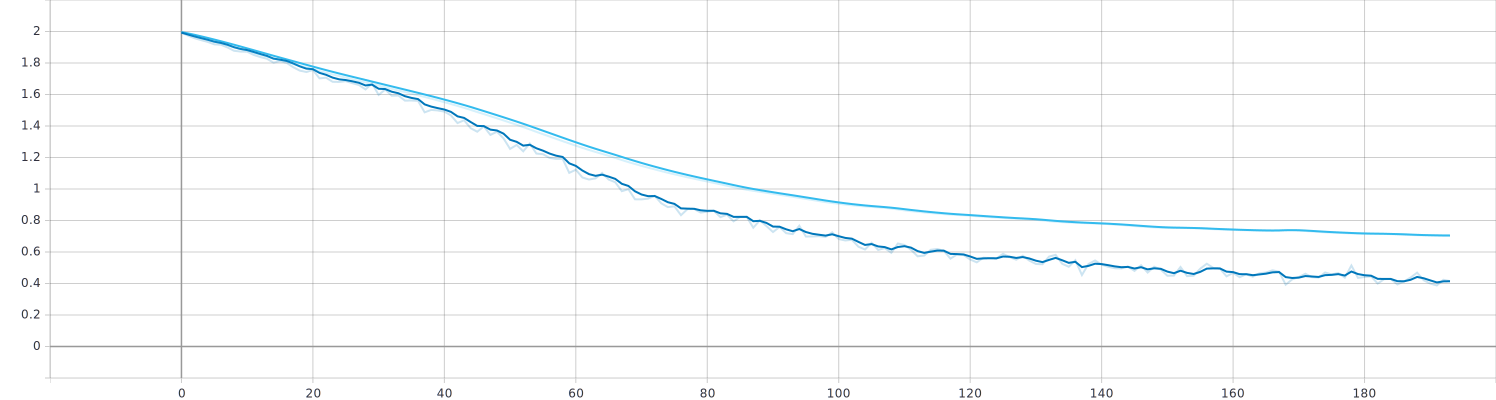
\includegraphics[width=0.7\linewidth]{results/fig/Loss3.png}
\caption{Loss graph}
\label{fig:evaluation3}
\end{figure}

\begin{figure}[htbp]
\centering
\includegraphics[width=0.6\linewidth]{results/fig/confusion3.png}
\caption{Confusion matrix}
\label{fig:confusion3}
\end{figure}

\chapter{Conclusion}

It seems that the slight modifications that I've tried did nothing to improve the model's accuracy. Indeed, the original model reports accuracy of 78.40\%, which tied with Ver. 2 and is strictly greater than the other two versions.

This accuracy is actually lower than the reported accuracy from Kipf \& Welling, which is actually 81.5\%.
I can't really explain why this is the case... But one guess is that maybe getting rid of the bias term might increase the accuracy? (<-- just a wild guess)

One interesting observation is that Ver. 3, the model with the most complexity out of the 4 tested, performed the worst with accuracy 77.54\%. It shows that adding in feature/model complexity doesn't always increase the accuracy; it might even decrease it!

\notecite{}
\printbibliography 
%\bibliographystyle{unsrt}
%\bibliography{bibs/references}
\addcontentsline{toc}{chapter}{Bibliography}

\end{document}